\documentclass[12pt, twoside]{report}

% Packages for equations and math symbols
\usepackage{amsmath}
\usepackage{amsfonts}
\usepackage{amssymb}

% Packages for figures
\usepackage{graphicx}
\usepackage{caption}
\usepackage{subcaption}
\usepackage{float}

% Packages for code
\usepackage{listings}
\usepackage{xcolor}

% Packages for links
% \usepackage{hyperref}
% \hypersetup{colorlinks=true,linkcolor=blue}

\definecolor{codegreen}{rgb}{0.1,0.6,0.1}
\definecolor{codegray}{rgb}{0.3,0.3,0.3}
\definecolor{codepurple}{rgb}{0.68,0,0.82}
\definecolor{backcolour}{rgb}{0.94,0.95,0.95}

% Python
\lstdefinestyle{python}{
    language=Python,
    backgroundcolor=\color{backcolour},
    commentstyle=\color{codegreen},
    keywordstyle=\color{magenta},
    numberstyle=\tiny\color{codegray},
    stringstyle=\color{codepurple},
    basicstyle=\linespread{1.0}\ttfamily\footnotesize,
    breakatwhitespace=false,
    breaklines=true,
    captionpos=b,
    keepspaces=true,
    numbers=left,
    numbersep=5pt,
    showspaces=false,
    showstringspaces=false,
    showtabs=false,
    tabsize=2,
}

\lstdefinestyle{inlinepython}{
    language=Python,
    basicstyle=\ttfamily\small,
    commentstyle=\color{codegreen},
    keywordstyle=\color{magenta},
    stringstyle=\color{codepurple},
    showstringspaces=false,
}

% Pseudocode
\lstdefinelanguage{Pseudocode}{
  morekeywords={for, to, end, if, then, else, while, do, repeat, until, return},
  morecomment=[l]{\#},
  morestring=[b]',
  sensitive=true
}
\lstdefinestyle{pseudocode}{
    language=Pseudocode,
    basicstyle=\ttfamily,
    keywordstyle=\bfseries,
    commentstyle=\itshape,
    xleftmargin=2em,
    aboveskip=1em,
    belowskip=1em,
}


% Double spacing
\usepackage{setspace}
\doublespacing

% Times New Roman font
\usepackage{times}

% Page margins
\usepackage[margin=1in]{geometry}

\begin{document}

% Title page
\title{CS 8770 \\ Neural Networks \\ Project 2}
\author{Drew Dahlquist \\ dgdtx5}
\date{April 25, 2023}
\maketitle

% Table of contents
\tableofcontents

% List of figures and tables (optional)
% \listoffigures
% \listoftables

% Chapter 1: Introduction
% \chapter{Introduction}

% Chapter 2: Technical Description
\chapter{Technical Description}

\section{Introduction}

For this project I decided to implement and explore LSTMs and find a dataset that naturally lends itself to 
sequence processing. I was able to find a decent quality dataset
\footnote[1]{https://archive.ics.uci.edu/ml/datasets/bike+sharing+dataset}
from the UCI Machine Learning repository on
bike sharing data that provides various features and the count of people who rented bikes for every hour over the 
span of 2 years, which gave me a good amount of data to work with, although of course more data would've been nicer.
In terms of getting started, I used a short PyTorch LSTM tutorial
\footnote[2]{https://pytorch.org/tutorials/beginner/nlp/sequence\_models\_tutorial.html}
to get my model class going, wrote the dataset class and data loaders by myself, and
salvaged my training loop from the last project.

I had a good amount of questions I wanted to attempt to answer during this project concerning LSTMs, as I'm
personally not very invested in predicting how many people will use bike sharing in a given hour.
I really wanted to build a good intution for designing and training LSTMs, particularly around how the
sequence length fed into the network influences training and inference, how the dimension of the cell/hidden states
influences the same as well as possibly gaining insight into what's going on in these mysterious features of LSTMs.
I looked into both some very natural ways for answering these questions 
(e.g., train, changing a hyperparameter, then train again) as well as some more exotic routes with the hopes
of finding them informative.

\section{Networks}

For my project I decided to study Long Short-Term Memory (LSTM) networks which are a type of 
recurrent neural network (RNN) architecture.
Unlike traditional RNNs, LSTMs can store information over longer periods of time, allowing them to better 
capture long-term dependencies in sequential data through the introduction of clever techniques allowing
gradients to better flow through the network without necissarily vanishing or exploding as is often the case
in traditional, vanilla RNNs.

At a high level, an LSTM module consists of several memory cells, which are responsible for storing information, 
and three gates - input, forget, and output gate - which control the flow of information into and out of the memory cells.
The forget gate determines which parts of the previous memory cells to forget.
It takes as input the current input, the previous hidden state, and a bias term, and produces an output between 0 and 1 
for each element of the memory cells.
The output ranging from 0 to 1 is then multiplied by the previous cell state resulting in the `forget' action 
(for values $< 1$).
Next the input gate determines which parts of the input to let through to the memory cells.
It takes as input the current input, the previous hidden state, and a bias term, and produces an output between 0 and 1 
for each element of the input.
This output is then multiplied by the candidate values and added to the current memory cells.
Lastly, the output gate determines which parts of the memory cells to output as the hidden state.
It takes as input the current input, the previous hidden state, and a bias term, and produces an output between 0 and 1 
for each element of the memory cells.
This output is then multiplied by the current memory cells passed through a non-linear activation function to 
produce the hidden state.
When stringing together multiple LSTM modules, the cell states and hidden states are fed into the following LSTM
as they are at this point and the process continues.

The equations for the input gate, forget gate, and output gate in PyTorch are as given below:

\begin{align}
    i_t &= \sigma(W_{ii} x_t + b_{ii} + W_{hi} h_{t-1} + b_{hi}) \\
    f_t &= \sigma(W_{if} x_t + b_{if} + W_{hf} h_{t-1} + b_{hf}) \\
    o_t &= \sigma(W_{io} x_t + b_{io} + W_{ho} h_{t-1} + b_{ho})
\end{align}

Where $x_t$ is the current input, $h_{t-1}$ is the previous hidden state, and $W_{**}$ and $b_{**}$ 
are the weight matrices and bias terms.
LSTMs then compute the candidate values for the memory cells as follows:

\begin{align}
    g_t = \tanh(W_{ig} x_t + b_{ig} + W_{hg} h_{t-1} + b_{hg})
\end{align}

Finally, the new memory cells and hidden state are computed as follows:

\begin{align}
    c_t &= f_t \odot c_{t-1} + i_t \odot g_t \\
    h_t &= o_t \odot \tanh(c_t)
\end{align}

While necessary for properly defining/training an LSTM, these equations feel more at home in a diagram of LSTMs,
illustrating just how the flow of information is gated/connected within each module.
From the below figure we easily see how the cell state gets update by means of passing the
previous hidden state through the various gates, as well how the cell state influences the outgoing
hidden state. A key feature of LSTMs is the `gradient highway' afforded to the cell state which allows
gradients to backpropagate through many LSTM modules relatively untouched, making training much less painful
than with vanilla RNNs.

\begin{figure}[H]
    \centering
    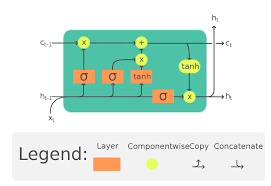
\includegraphics[width=0.75\textwidth]{figures/lstm fig.png}
    \caption*{LSTM (source: wikipedia.com)}
\end{figure}

\section{Data}

The dataset used is the Bike Sharing dataset coming from the UCI Machine Learning repository. The dataset consists of
two files containing various information such as date, season, year, weather, and most importantly, the
number of bikes rented by the hour or day (depending on which file you look at). For my project I chose
to use the hour.csv file only as this would allow me to pull more sequences for both training and testing.
I also did some manual feature selection via Microsoft Excel, and threw out some of the features I felt were
unnecessary such as instant, casual, registered, etc. In the end I was left with 11 features and 1 target variable –
the total count of riders during a given hour.

The main method of inference I focused on was given some sequence of previous hours, try to best predict the 
number of users that would rent bikes within the next hour. Although simple to state, this actually provided more
than enough material to work with in terms of exploring the internals of LSTMs, trying to answer some natural questions
I had going into this project, and also actually training a good network for perdiction.

In order to accomplish the above, I created my own custom PyTorch dataset class, which handles reading in the csv,
holding information about the sequence length being used, size of the data set, and retrieval of (feature, target) pairs - 
which in this case are sequences of the 11 features and the true count of users over the next hour.
For training/testing I stuck with a 4-to-1 ratio as I needed as much data for training as possible, and only
roughly cared about validation/testing for this project. As I discuss later in the project, while the LSTM
could properly learn, the data had a sufficient amount of noise so as to make highly accurate prediction very difficult.
However, the accuracy was still plenty close to notice the network was properly learning and to be an overall
acceptable machine.

\section{Training}

In an RNN, the same set of weights is used at each time step to process the current input and the previous hidden state.
As a result, the gradients that are computed during backpropagation must be propagated through time to all previous 
time steps in order to update the weights properly since the error at a given time step may depend on the 
inputs and hidden states from many previous time steps.

This is addressed via backprop through time (BPTT) by unrolling the RNN for a fixed number of time steps during training, 
creating a `deep' feedforward neural network with shared weights at each time step.
The gradients are then computed for each time step using the standard backpropagation algorithm, 
and the weights are updated using via optimization which is familiar from simpler MLPs or CNNs.

The unrolling process involves creating a copy of the RNN for each time step, and connecting the hidden state at 
one time step to the input at the next time step.
This creates a `chain' of RNNs that are connected through time and leads to the very cleverly named algorithm 
called `backpropagation through time'.
In theory this is perfect, however it causes some computational difficulties during training as it may lead to
the gradients becoming very small or very large as they are propagated through the many layers of the unrolled net,
making it difficult or impossible to update the weights properly.
This is known as the `vanishing gradient' and `exploding gradient' problems, respectively.

There are many ways to address this issue with gradients during training such as gradient clipping, different
activation functions, or by model respecification (i.e., LSTMs).
LSTMs address this key difficulty in training RNNs through the use of its gating mechanisms.
These mechanisms allow the network to selectively `remember' and `forget' information over time, 
which ideally prevents the gradients from becoming too small or too large during training.
Specifically, this is where LSTMs three gates - input, output, and forget gates - come in to play so as to 
control the flow of information through the network.
The input gate controls which information should be added to the cell state, while the forget gate decides 
which information should be discarded, and the output gate controls the output that is generated by the network.
Through the means of these gates, LSTMs can selectively update or ignore information at each time step,
which helps to prevent the gradients from vanishing or exploding as in vanilla RNNs.

% Chapter 3: Experiments and Results
\chapter{Experiments and Results}

\section{Sanity Check}

Before getting into the finer details of LSTMs, I wanted to ensure that my model was functioning in good order.
Besides watching training and validation loss decrease during training I figured it'd be good to manually inspect
some of the inner workings to save my sanity as I got further along in the project as well as to strengthen my 
understanding of how to navigate around LSTMs practically.
I started by manually verfying the predicted counts were at least roughly near the true counts, as I wasn't
expecting perfect performance but would like to be able to claim some level of accuracy in my model.
I ran this check a few times during and after training with randomly selected samples and eyeballed the outcome, an
example is shown below which comes from a trained LSTM and is good enough for me.

\begin{lstlisting}[style=Python,caption=Sample preds vs labels,label=lst:python]
    predictions = tensor([320.1914, 345.4972,  ..., 164.6243, 193.7517])
    labels      = tensor([385.    , 401.    ,  ..., 167.    , 210.])
\end{lstlisting}

Next I decided to ensure the distribution of predictions was more or less in-line with that of the true labels.
Again the below density plot from a trained LSTM checks out. It should be noted that while having these
densities perfectly match would be necessary for a strong model, it's not sufficient as we still care about 
which samples predict which values, not just that the total distribution of values matches.
While there are plenty more tests I could've ran to ensure the quality of my data, model, training, etc.
these two quick checks gave me enough confidence in my model and training loop to proceed and have faith
that my resulting conclusions stood on firm ground.

\begin{figure}[H]
    \centering
    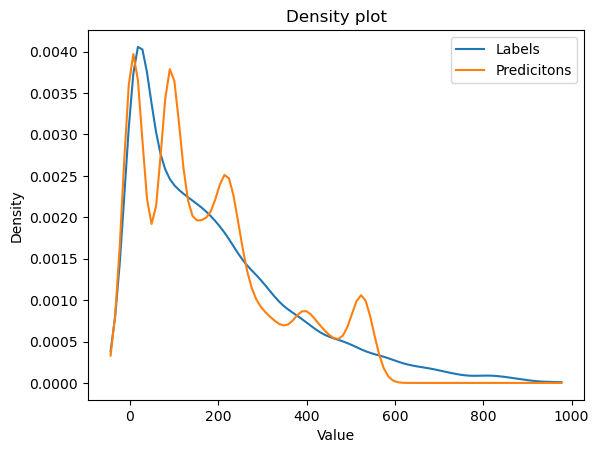
\includegraphics[width=0.65\textwidth]{figures/density plot.png}
    \caption*{Density of true vs pred counts}
\end{figure}

\section{Sequence Length}

One of the first questions I had when starting to work with LSTM's was exactly what effect
the sequence length being fed into the network would have on the resulting inference. Intuitively,
it feels like our predictions should only get better as we feed in more prior data, since having a longer
sequence only adds information. However, I was still uncertain whether this would even be close to true,
since there are a lot of mechanics inside LSTMs that the presence of more sequential information may tamper
with.

In order to experiment with the effective of sequence length, I trained my LSTM until convergence with all
the same hyperparameters (hidden dim $= 5$, etc.) but only varied how many elements of the sequence I fed into it
for training and testing. Due to the hourly nature of my data, I opted to block of sequence length in natural intervals
such as 8 hours, 24 hours, etc. as it seemed the most natural considering its a time series. The results of this 
experiment is shown in the below plot.

\begin{figure}[H]
    \centering
    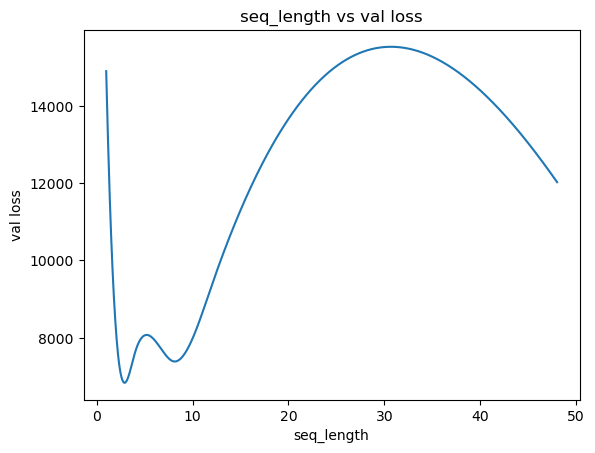
\includegraphics[width=0.75\textwidth]{figures/seq len vs val loss.png}
    \caption*{seq len vs val loss}
\end{figure}

It's easily seen my hypothesis of performance increasing with sequence length clearly didn't hold.
The initial decrease in val loss was entirely expected, as it's much easier to predict the next value
given the previous 2,4, or even 8, as opposed to just the previous 1.
What I wasn't planning on seeing was the sharp increase in val loss as the sequence length increases.
Furthermore, the decrease in validation loss after around 30 is most likely due to random variation from 
model initialization or train-validation splitting and not due to sequence lenght.

After some thought I feel the most likely explanation is that the longer sequence length affects the dynamics
of BPTT in a negative way resulting in more difficult training and thus worse performance on the validation set.
Ideally I would've liked to have multiple runs for each sequence length in order to marginalize any
effects from random initialization, randomization in batch presentation, and other conditions that generally
have little to nothing to do with the sequence length. However, training times on my laptop were much too long
to continue rerunning the same experiment to nail down a precise answer for optimal sequence length, so I took
the above conclusion of `it depends' as good enough and moved on.

\section{Hidden Dimension}

The next natural question I had was what effect does the hidden dimension have on the LSTMs
ability to both learn and performance inference. Intuitively I was expecting learning capacity to peak 
somewhere within $4 < h < 20$ (equivalently min. val. loss) as I figured this would provide enough space 
for the LSTM to `organize'  the infomartion in terms of cell state and hidden state yet would still be small 
enough that training is effective as considering the extreme of, say, $500$ hidden dimensions feels 
like it would hurt more than help.
The below figure plots the loss on a validation set for varying hidden dimension's between 1 and 40.
I opted to not see what happens fully training an LSTM with 500 hidden dimensions as 1 epoch took roughly 3 
minutes to train on my laptop - I feel like 40 is plenty high of an upper bound for these experiments.

\begin{figure}[H]
    \centering
    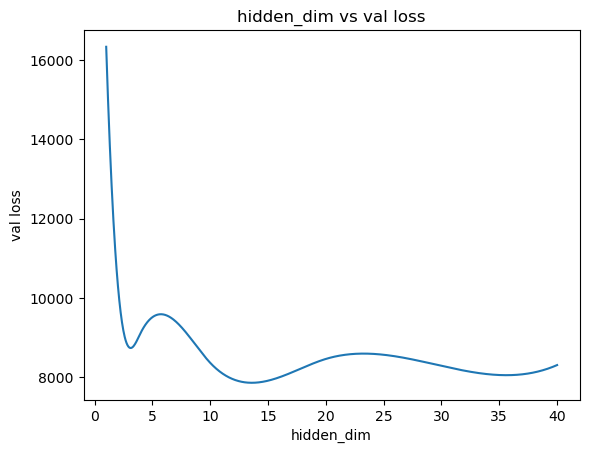
\includegraphics[width=0.65\textwidth]{figures/hidden dim vs val loss.png}
    \caption*{hidden dim vs validation loss}
\end{figure}

However, I still wanted to test my theory of whether more dimensions was affording the LSTM the ability
to better `organize its thoughts'.
I started with an LSTM with hidden dim $= 2$ to be able to easily visualize the cell state and hidden state 
for all samples fed into the net with a scatter plot colored by the true count value. This plot is shown below.
Qualitatively, this looks to be exactly the case as the LSTM is doing a good job to organize samples 
with similar count values into similar areas of its hidden space, both via cell state and hidden state.
Of these two, the cell state was the most surprising as there's nowhere I'm directly optimizing it, 
whereas the hidden states final output in the sequence is fed into a linear layer to produce a prediction and is
thus directly in line with the loss function.

\begin{figure}[H]
    \centering
    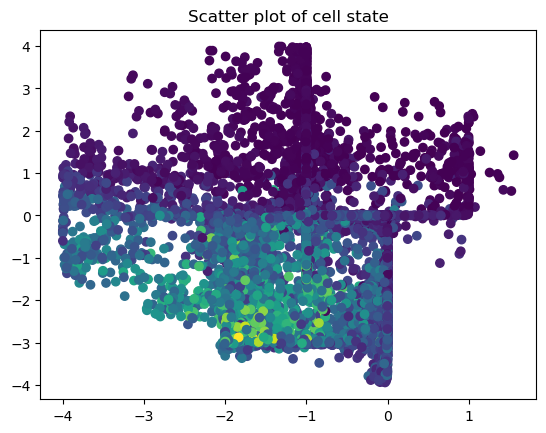
\includegraphics[width=0.65\textwidth]{figures/dim 2 cell state.png}
    \caption*{Visualization of 2 dimensional cell state colored by true count value}
\end{figure}

\begin{figure}[H]
    \centering
    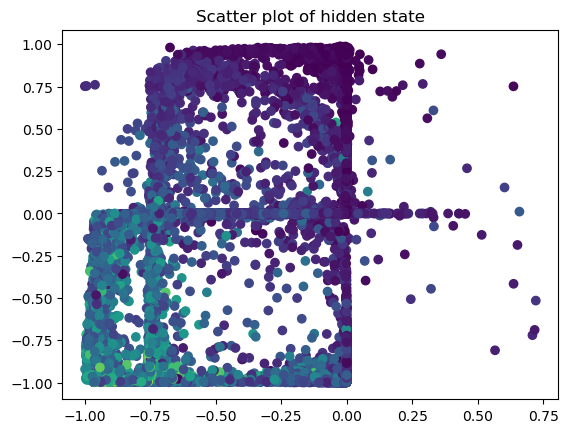
\includegraphics[width=0.65\textwidth]{figures/dim 2 hidden state.png}
    \caption*{Visualization of 2 dimensional hidden state colored by true count value}
\end{figure}

Looking into 2 dimensions was interesting enough to merit some more investigation into this feature,
yet visualizing 3 dimensions on a computer is clumsy and $\geq$ 4 dimensions is impossible.
Therefore I decided to reduce the dimesnion of the cell states and hidden states (after training/inference)
for visualization via t-SNE. The below two plots are exactly this reconstruction of the previous two 
with another trained LSTM with hidden dimension $= 4$.
While t-SNE isn't perfect, we can still see a lot of the same behavior where
counts with similar values are clumped together and counts with very different values tend to be much further.

\begin{figure}[H]
    \centering
    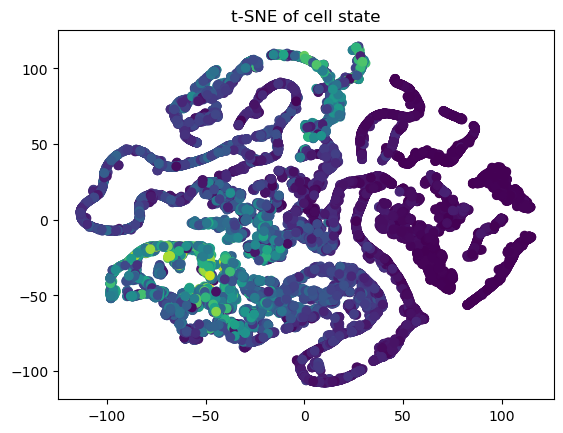
\includegraphics[width=0.65\textwidth]{figures/dim 4 cell state.png}
    \caption*{Visualization of 4 dimensional cell state colored by true count value}
\end{figure}

\begin{figure}[H]
    \centering
    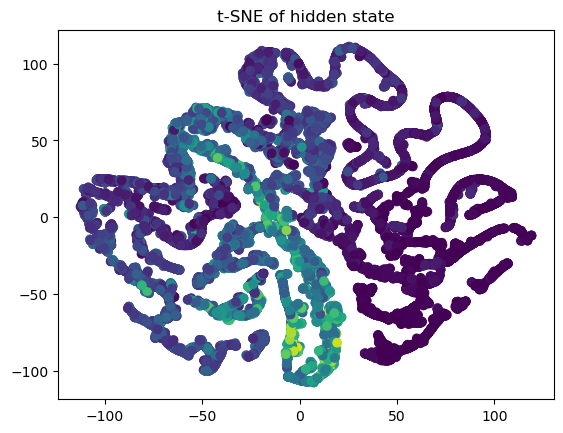
\includegraphics[width=0.65\textwidth]{figures/dim 4 hidden state.png}
    \caption*{Visualization of 4 dimensional hidden state colored by true count value}
\end{figure}

\section{Visual Dimension}

The above results regarding peeking into the cell state and hidden state really interested me,
so instead of just looking at the fully trained result I decided to collect some visuals throughout
the training process, hoping to see the organizational pattern mentioned previously slowly emerge.
The below are visualizations of the high-dimensional cell state using t-SNE over the course of training the LSTM.
Each individual point is a prediction from the network on validation data and is colored according to the 
magnitude of the true label as before.
The corresponding figures for hidden state are similar, therefore I'm only showing cell state since it surprised me
the most as the setup of the LSTM places little emphasis on what exactly the cell state does, so long as its final
feed into the hidden state and resulting inference is more or less useful.

\begin{figure}[H]
    \centering
    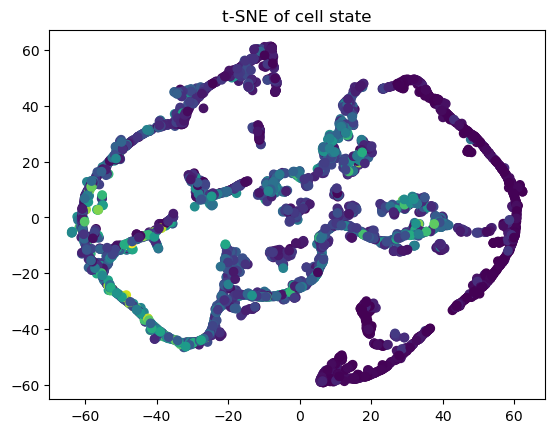
\includegraphics[width=0.65\textwidth]{figures/cell state evolution/1 epoch.png}
    \caption*{t-SNE of Cell State After 1 epoch}
\end{figure}

\begin{figure}[H]
    \centering
    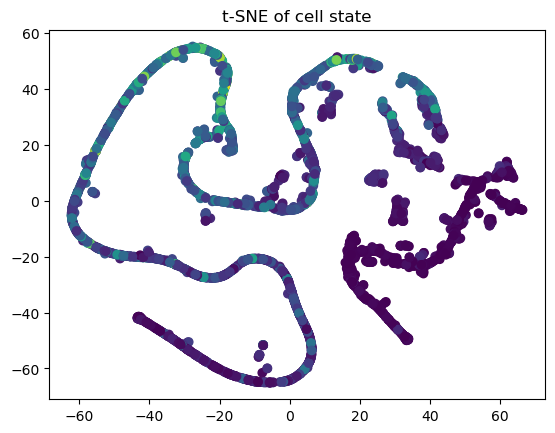
\includegraphics[width=0.65\textwidth]{figures/cell state evolution/3 epoch.png}
    \caption*{t-SNE of Cell State After 3 epoch}
\end{figure}

\begin{figure}[H]
    \centering
    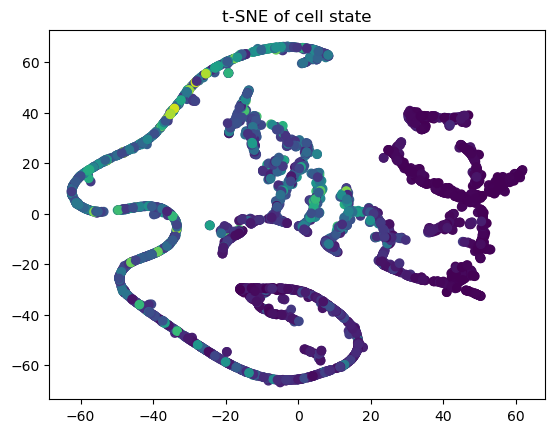
\includegraphics[width=0.65\textwidth]{figures/cell state evolution/5 epoch.png}
    \caption*{t-SNE of Cell State After 5 epochs}
\end{figure}

\begin{figure}[H]
    \centering
    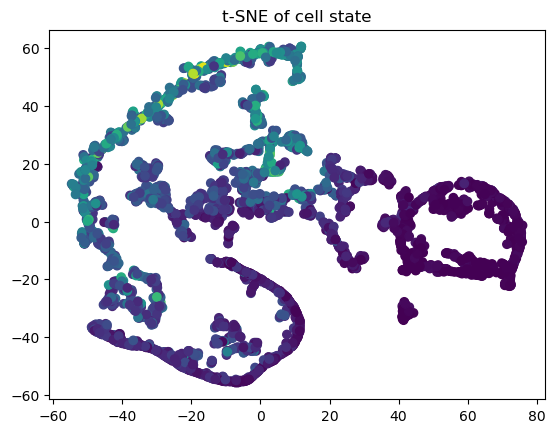
\includegraphics[width=0.65\textwidth]{figures/cell state evolution/15 epoch.png}
    \caption*{t-SNE of Cell State After 15 epochs}
\end{figure}

Personally, the above figures wow'd me. It makes sense that the cell state and hidden state would organize
samples that require a similar predicted value into similar areas of space - somewhat similar to word embeddings -
but to the extent that these come from my tiny LSTM trained on my tiny laptop using a (all things considerd) tiny dataset
was remarkable I thought.
There really isn't a whole lot of useful insight I can really provide on the above besides a bunch of
conjectures on why this property occurs.
My most likely explanation is that at initialization, the LSTM is predicting all of the counts to be near 0
(i.e., all equally wrong in the same way), so during optimization the larger count values produce a larger 
loss and therefore a larger gradient, where the smaller values do the opposite. This, coupled with the fact
there is some hidden structure in this dataset (e.g., more people ride bikes in summer than winter)
results in the training samples also being very similar themselves, causing the LSTM gates to fire in 
much the same way. However, I couldn't really do much to test out this theory as it's something that needs to be
marginalized over multiple datasets and inference tasks, but its my best guess.

% Chapter 4: Reflection
\chapter{Reflection}

Working with LSTMs in PyTorch was a challenging but useful experience for me overall.
At the start of working on this proejct the amount of time it took to set up the dataset and dataloader
for sequence processing was a bit surprising as it presented some unexpected overhead setting up properly
for training / testing splits. However, it was all pretty straightforward, it just required some extra time and care
since its the foundation of training an RNN.
Especially when compared to MNIST classification, where the data is already in a straightforward format,
sequence data required more preprocessing and formatting.

I also felt that training LSTMs is more `touchy' than training MLPs or CNNs
since LSTMs are a more complex type of neural network, with more parameters and more fine-tuning required.
I found that getting the right hyperparameters and tuning the model took a lot of trial and error as well as time
since iterating on LSTMs isn't cheap for a CPU.
However, I also suspect that some training difficulties may be partially due to the specific dataset I used, 
and I'd like to experiment with other datasets to see if this is really the case - my gut says yes but 
I'm unsure to what extent.

Despite the challenges, I enjoyed exploring some of the potential of RNNs / LSTMs.
I would've really liked to have had more time to apply LSTMs to other applications they've proven to be effective at like
image captioning, machine translation, and some small language modeling.
I think it would've been great to get into some of these as it sort of `marginalizes' the application / data specific 
features and I would've walked away understanding LSTMs a bit better in terms of their low-level mechanics and also
the heuristics for when and how to apply them to different problems.

I also wish this project allocated some time / incentive to starting with vanilla RNNs before moving on to LSTMs.
I would've enjoyed to explore the internals of training vanilla RNNs and finding all their pain points, then moving
to LSTMs and (hopefully) see the issues with training vanilla RNNs (e.g., gradient troubles) go away, since in my mind
LSTMs came about in order to `fix' some problems with vanilla RNNs.

Overall, I really enjoyed working with RNNs and sequence processing. These models gave much more content to grab
onto for exploring didn't feel as `basic' as MLPs/CNNs for MNIST image classification and have left me wanting to do
more with them.

% References
\bibliographystyle{plain}
\bibliography{references}


\end{document}
